\documentclass[11pt]{article}
\usepackage{setspace}
\usepackage[a4paper,margin=1in]{geometry}
\geometry{margin=0.85in}
\setstretch{1.0}
\usepackage{graphicx}
\usepackage{array}
\usepackage{setspace}
\usepackage{parskip}
\usepackage{ragged2e}

\pagestyle{empty}
\setstretch{1.05}

\begin{document}


% Title
\begin{center}
    {\Large \textbf{Bewerbung}} \\[3cm]
    
    {\Huge \textbf{Zhongli Wang}} \\[0.4cm]
    
    {\huge Bewerbung als Leitung FDZ und Co-Leitung Cluster}
\end{center}

\vspace{0.6cm}

% Large picture in the middle
\begin{center}
    \IfFileExists{../zhongli-wang-profile.jpg}{
        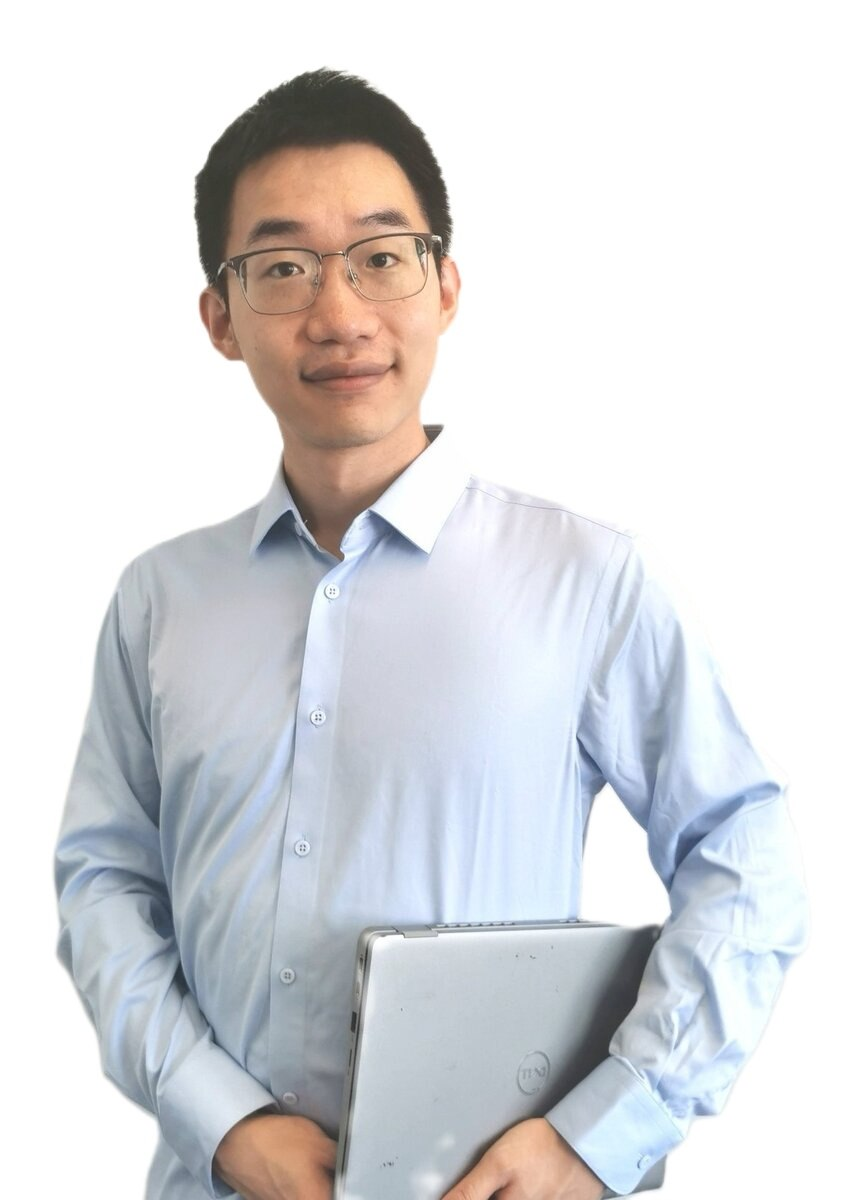
\includegraphics[
            width=0.55\textwidth,
            height=0.45\textheight,
            keepaspectratio
        ]{../zhongli-wang-profile.jpg}
    }{
        \vspace{0.45\textheight}
    }
\end{center}

\vspace{0.7cm}

% \vspace{3cm}


% Personal details
\begin{center}
\renewcommand{\arraystretch}{1.35}
\begin{tabular}{>{\bfseries}p{4.2cm} p{8.5cm}}

Anschrift: & Astastrasse 22, 33617 Bielefeld, Germany \\

Telefon: & +49 160 9541 6015 \\

E-Mail: & nkwangzhongli@gmail.com \\
\end{tabular}
\end{center}

\vfill

% \begin{center}
%     \small Last updated: \today
% \end{center}
\newpage
\enlargethispage{4\baselineskip}

\begin{flushright}
Zhongli Wang \\
+49 160 9541 6015 \\
nkwangzhongli@gmail.com \\
Bielefeld, Germany \\
\end{flushright}

\vspace{0.1cm}

\noindent
Dr. Jannes Jacobsen \\
DeZIM-Institut \\
Cluster „Daten-Methoden-Monitoring“ und FDZ \\

\vspace{0.1cm}

\noindent
Bewerbung auf die Kennziffer PR/09/26 \\

\vspace{0.05cm}

\noindent Sehr geehrter Herr Dr. Jacobsen,

hiermit bewerbe ich mich auf die Position Leitung Forschungsdatenzentrum und Co-Leitung des Clusters „Daten – Methoden – Monitoring“ am DeZIM-Institut. Ich befinde mich in der Abschlussphase meiner Promotion in Economics an der Universität Bielefeld, meine Verteidigung ist für den 21. September 2026 terminiert. Inhaltlich verbinde ich quantitative Sozialforschung, Computational Social Science, Forschungsdatenarbeit und internationale Zusammenarbeit.

Besonders passend finde ich die Verbindung aus Dateninfrastruktur, Methodenberatung und eigenständiger Forschung. In meiner Dissertation entwickle ich agentenbasierte und spieltheoretische Modelle zu digitalen Märkten, heterogenen Akteuren und datengetriebenen Wertschöpfungsketten. Dabei arbeite ich mit Python, R, Julia, Mathematica, SMM, MCMC und maschinellem Lernen, dokumentiere Modellannahmen reproduzierbar und übersetze komplexe Ergebnisse in klare Publikationen und Vorträge.

Für die ausgeschriebene Querschnittsaufgabe bringe ich insbesondere folgende Stärken mit:

\begin{itemize}
    \item \textbf{Methoden:} Computational Social Science, ABM, Ökonometrie, ML und Simulationen.
    \item \textbf{Forschungsdaten:} Aufbereitung, Strukturierung und Dokumentation von Daten, Modellen und Code für nachvollziehbare Analysen.
    \item \textbf{Kommunikation:} Lehr- und Assistenzarbeit in quantitativer Betriebswirtschaftslehre sowie internationale Konferenzvorträge.
    \item \textbf{Koordination:} Internationale Forschungsprojekte, Workshop-Organisation und Zusammenarbeit mit verschiedenen Disziplinen.
\end{itemize}

Inhaltlich sehe ich Anschluss an DeZIM-relevante Fragen zu Teilhabe, Ungleichheit und datenbasiertem Monitoring. Mein Projekt zu „Heterogeneous Consumers and the Data Value Chain“ untersucht, wie Datenrestriktionen räumliche Marktdynamiken und heterogene Akteursgruppen beeinflussen. Diese Perspektive würde ich gerne in Forschungsdateninfrastrukturen, Metadatenarbeit und methodische Beratung einbringen.

Meine bisherige Erfahrung liegt stärker in quantitativer Forschung, Modellierung und Forschungsorganisation als in der formalen Leitung eines Forschungsdatenzentrums. Die Leitungsaufgabe würde ich daher mit einem kooperativen, dokumentationsstarken und lernorientierten Arbeitsstil angehen. Mit meiner deutschen Sprachkompetenz, meiner internationalen Forschungserfahrung und meinem methodischen Profil kann ich das Cluster fachlich und organisatorisch unterstützen.

Vielen Dank für die Prüfung meiner Bewerbung. Ich freue mich über die Möglichkeit, meine Eignung und meine Ideen für die Weiterentwicklung des DeZIM.fdz im Gespräch zu erläutern.

\vspace{0.05cm}
\noindent Mit freundlichen Grüßen \\[0.08cm]
\noindent Zhongli Wang \\[-0.35cm]

\vspace{0.1cm}
\noindent
\includegraphics[height=0.75cm,keepaspectratio]{../Wang-sig.jpg}

\end{document}
